\documentclass[12pt]{article}
\usepackage{amsmath, amssymb, amsfonts, amsthm, mathtools,mathrsfs}
\usepackage{thmtools}
\usepackage[utf8]{inputenc}
\usepackage[inline]{enumitem}
\usepackage[colorlinks=true]{hyperref}
\usepackage{tikz}
\usetikzlibrary{decorations.markings}
\usetikzlibrary{arrows.meta}
\usepackage{witharrows}
\usepackage{datetime2}

\setlength\parindent{0pt}
\usepackage{parskip}

\usepackage[framemethod=tikz]{mdframed}
\mdfdefinestyle{theoremstyle}{%
	% linecolor=gray,linewidth=1pt,%
	% frametitlerule=true,%
	frametitlebackgroundcolor=white,
	% backgroundcolor=  gray!20,	
	bottomline=false, topline=false, rightline=false, leftline=true,
	innerlinewidth=0.7pt, outerlinewidth=0.7pt, middlelinewidth=2pt, middlelinecolor=white, %
	innerleftmargin=6pt,
	% innertopmargin=-1pt,
	skipabove=10pt,
	% fontcolor=blue,
	% innerbottommargin=-0.5pt,
}
\mdtheorem[style=theoremstyle]{defn}[thm]{Definition}
\mdtheorem[style=theoremstyle]{thm}{Theorem}

\newcommand*{\doublerule}{\hrule width \hsize height 1pt \kern 0.5mm \hrule width \hsize height 2pt}
\newcommand{\doublerulefill}{\leavevmode\leaders\vbox{\hrule width .1pt\kern1pt\hrule}\hfill\kern0pt}

\usepackage{xpatch}
\newcommand{\thmautorefname}{Theorem}
\makeatletter
\xpatchcmd{\thm}{\refstepcounter}{\NR@gettitle{#1}\refstepcounter}{}{}
\makeatother

\newcommand{\Res}{\operatorname{Res}}
\newcommand{\md}[1]{\left\lvert #1 \right\lvert}
\newcommand{\fl}[1]{\left\lfloor #1 \right\rfloor}

\theoremstyle{definition}
% \newtheorem{thm}{Theorem}
% \numberwithin{thm}{section}
% \newtheorem{lem}[thm]{Lemma}
% \newtheorem{defn}[thm]{Definition}
% \newtheorem{prop}[thm]{Proposition}
% \newtheorem{cor}[thm]{Corollary}
% \newtheorem{ex}{Example}


\let\emptyset\varnothing

\pagestyle{plain}

\usepackage{titlesec}
\titleformat{\section}[block]{\sffamily\Large\filcenter\bfseries}{\S\thesection.}{0.25cm}{\Large}
\titleformat{\subsection}[block]{\large\bfseries\sffamily}{\S\S\thesubsection.}{0.2cm}{\large}

\usepackage[a4paper]{geometry}
\usepackage{lipsum}

\usepackage{cleveref}
\crefname{thm}{Theorem}{Theorems}
\crefname{lem}{Lemma}{Lemmas}
\crefname{defn}{Definition}{Definitions}
\crefname{prop}{Proposition}{Propositions}
\crefname{cor}{Corollary}{Corollaries}
\crefname{equation}{}{}

\usepackage{mdframed}
\newenvironment{blockquote}
{\begin{mdframed}[skipabove=0pt, skipbelow=0pt, innertopmargin=4pt, innerbottommargin=4pt, bottomline=false,topline=false,rightline=false, linewidth=2pt]}
{\end{mdframed}}
\newenvironment{soln}{\begin{proof}[Solution]}{\end{proof}}

\usepackage{fancyhdr}
\setlength{\headheight}{15.2pt}
\pagestyle{fancy}
\fancyhf{}
\fancyhead[L]{\sffamily{\S\textbf{\nouppercase{\leftmark}}}}
\fancyhead[R]{\sffamily{\thepage}}
\definecolor{myupdatecolor}{RGB}{0, 0, 255}

% \usepackage{xcolor}
% \definecolor{mybgcolor}{RGB}{50, 50, 50} %46, 51, 63
% \usepackage{pagecolor}
% \pagecolor{mybgcolor}
% \color{white}
% \mdfsetup{backgroundcolor=mybgcolor, fontcolor=white}
% \definecolor{myupdatecolor}{RGB}{0, 255, 0}

\renewcommand{\familydefault}{\sfdefault}

\title{MA 109: Calculus I\\\large{Tutorial Solutions}}
\author{Aryaman Maithani\\\url{https://aryamanmaithani.github.io/tuts/ma-109}}
\date{Autumn Semester 2020-21\\~\\Last update: \DTMnow}

\begin{document}
\tikzset{lab dis/.store in=\LabDis,
  lab dis=-0.4,
  ->-/.style args={at #1 with label #2}{decoration={
    markings,
    mark=at position #1 with {\arrow{>}; \node at (0,\LabDis) {#2};}},postaction={decorate}},
  -<-/.style args={at #1 with label #2}{decoration={
    markings,
    mark=at position #1 with {\arrow{<}; \node at (0,\LabDis)
    {#2};}},postaction={decorate}},
  -*-/.style args={at #1 with label #2}{decoration={
    markings,
    mark=at position #1 with {{\fill (0,0) circle (1.5pt);} \node at (0,\LabDis)
    {#2};}},postaction={decorate}},
  }
\maketitle
\tableofcontents
\newpage
\setcounter{section}{-1}
\section{Notations}
\begin{enumerate}
	\item $\mathbb{N} = \{1,\; 2,\; \ldots\}$ denotes the set of natural numbers.
	\item $\mathbb{Z} = \mathbb{N} \cup \{0\} \cup \{-n : n\in\mathbb{N}\}$ denotes the set of integers.
	\item $\mathbb{Q}$ denotes the set of rational numbers.
	\item $\mathbb{R}$ denotes the set of real numbers.
	\item $\subset$ is used for subset, not necessarily proper.
	\begin{equation*} 
		[0, 1] \subset [0, 1]
	\end{equation*}
	is correct.
	\item $\subsetneq$ is used for ``proper subset.''
\end{enumerate}
\newpage\section{Tutorial 1}
\begin{center}
	25th November, 2020
\end{center}
\textbf{Sheet 1}
\begin{itemize}[leftmargin=*]
	\item [2. (iv)]$\displaystyle\lim_{n\to \infty}(n)^{1/n}.$

	Define $h_n \vcentcolon= n^{1/n} - 1.$\\
	Then, $h_n \ge 0$ for all $n \in \mathbb{N}.$ \hfill (Why?)

	Now, for $n > 2,$ we have 
	\begin{align*} 
		n &= (1 + h_n)^n \\
		&= 1 + nh_n + \dbinom{n}{2}h_n^2 + \cdots + \dbinom{n}{n}h_n^n\\
		&\ge 1 + nh_n + \dbinom{n}{2}h_n^2 \\
		&> \dbinom{n}{2}h_n^2 \\
		&= \dfrac{n(n-1)}{2}h_n^2.
	\end{align*}

	Thus, $h_n < \sqrt{\dfrac{2}{n-1}}$ for all $n > 2.$

	Using Sandwich Theorem, we get that $\displaystyle\lim_{n\to \infty}h_n = 0$ which gives us that 
	\begin{equation*} 
		\displaystyle\lim_{n\to \infty}n^{1/n} = 1.
	\end{equation*}

	(Where did we use that $h_n \ge 0?$)
	%
	\newpage
	\item[3. (ii)] We show that $\left\{(-1)^n\left(\dfrac{1}{2} - \dfrac{1}{n}\right)\right\}_{n \ge 1}$ is \emph{not} convergent.

	\begin{soln}
	
	Note that from the difference formula, we know that if $\{a_n\}$ converges, then
	\begin{equation*} 
		\lim_{n\to \infty}\left|a_{n+1} - a_n\right| = 0.
	\end{equation*}
	(The limit \emph{exists} and equals $0.$)

	We show that this is not true for the given sequence. We define 
	\begin{equation*} 
		b_{n} \vcentcolon= a_{n + 1} - a_n,
	\end{equation*}
	where $\{a_n\}$ is the sequence given in the question.	

	Then, $b_n$ is given as
	\begin{align*} 
		b_n &= (-1)^{n+1}\left(\dfrac{1}{2} - \dfrac{1}{n+1}\right) - (-1)^n\left(\dfrac{1}{2} - \dfrac{1}{n}\right)\\
		&= (-1)^{n+1}\left(\dfrac{1}{2} - \dfrac{1}{n+1}\right) + (-1)^{n+1}\left(\dfrac{1}{2} - \dfrac{1}{n}\right)\\
		&= (-1)^{n+1} + (-1)^{n}\left(\dfrac{1}{n+1} + \dfrac{1}{n}\right).
	\end{align*}
	Thus, we have
	\begin{align*} 
		|b_n| &= \left|1 - \left(\dfrac{1}{n+1} + \dfrac{1}{n}\right)\right|\\
		&= \left|1 - \dfrac{2n + 1}{n(n + 1)}\right|
	\end{align*}
	From the above, we conclude that
	\begin{equation*} 
		\lim_{n\to \infty}|b_n| = 1.
	\end{equation*}
	This shows that $a_n$ does not converge.
	\end{soln}
	%
	\newpage
	\item[5. (iii)] $a_1 = \sqrt{2},\;a_{n+1} = 3 + \dfrac{a_n}{2} \quad \forall n \ge 1.$
	\begin{soln}
		I first describe the general idea.\\

	\begin{blockquote}
		The idea in these questions is to first prove a bound on $a_n$ by induction. Then, using that bound we prove that the sequence is convergent.

		Once we do that, we then know that $\lim_{n\to \infty}a_n$ exists. Since that also equals $\lim_{n\to \infty}a_{n+1},$ we can take limit on both sides of the equation and solve for the limit $L.$
	\end{blockquote}

	First, we prove that the sequence is bounded above.\\

	\begin{blockquote}
	Claim 1. $a_n < 6$ for all $n \in \mathbb{N}.$ 
	\begin{proof} 
		We shall prove this via induction. The base case $n = 1$ is immediate as $2 < 6.$\\
		Assume that it holds for $n = k.$ Then,
		
		\begin{equation*} 
			a_{k+1} = 3 + \dfrac{a_n}{2} < 3 + \dfrac{6}{2} = 6.
		\end{equation*}

		By principle of mathematical induction, we have proven the claim. 
	\end{proof}
	\end{blockquote}
	\phantom{hi}
	\begin{blockquote}
	Claim 2. $a_n < a_{n+1}$ for all $n \in \mathbb{N}.$ 
	\begin{proof} 
		$a_{n+1} - a_n = 3 - \dfrac{a_n}{2} = \dfrac{6 - a_n}{2} > 0 \implies a_{n+1} > a_n.$ 
	\end{proof}
	\end{blockquote}

	Thus, we now know that the sequence converges. Let $L = \lim_{n\to \infty}a_n.$ Then taking the limit on both sides of
	\begin{equation*} 
		a_{n+1} = 3 + \dfrac{a_n}{2}
	\end{equation*}
	gives us
	\begin{equation*} 
		L = 3 + \dfrac{L}{2},
	\end{equation*}
	which we can solve to get $L = 6.$
	\end{soln}
	%
	\newpage	
	\item[7.] If $\displaystyle\lim_{n\to \infty}a_n = L \neq 0,$ show that there exists $n_0 \in \mathbb{N}$ such that
    \begin{equation*} 
    	|a_n| \ge \dfrac{|L|}{2} \quad \text{ for all } n \ge n_0.
    \end{equation*}

    \begin{soln}
    	Choose $\epsilon = \dfrac{\left|L\right|}{2}.$ Note that this is indeed greater than $0.$

    	By the $\epsilon-N$ definition, there exists $N \in \mathbb{N}$ such that
    	\begin{equation*} 
    		|a_n - L| < \epsilon = \dfrac{|L|}{2}
    	\end{equation*}
    	for all $n > N.$ Using triangle inequality, we get
    	\begin{equation*} 
    		||a_n| - |L|| \le |a_n - L| < \dfrac{|L|}{2}.
    	\end{equation*}
    	Thus, we get
    	\begin{equation*} 
    		-\dfrac{|L|}{2} < |a_n| - |L| < \dfrac{|L|}{2}.
    	\end{equation*}
    	Adding $|L|$ on both sides gives us
    	\begin{equation*} 
    		\dfrac{|L|}{2} < |a_n| < \dfrac{3|L|}{2}
    	\end{equation*}
    	for all $n > N,$ as desired.
    \end{soln}
    %
    \newpage
    \item[9.] For given sequences $\{a_n\}_{n \ge 1}$ and $\{b_n\}_{n \ge 1},$ prove or disprove the following:
    \begin{enumerate}
    	\item $\{a_nb_n\}_{n \ge 1}$ is convergent, if $\{a_n\}_{n \ge 1}$ is convergent.
    	\item $\{a_nb_n\}_{n \ge 1}$ is convergent, if $\{a_n\}_{n \ge 1}$ is convergent and $\{b_n\}_{n \ge 1}$ is bounded.
    \end{enumerate}
    \begin{soln}
    	Both the statements are false. We give one counterexample for both.
    	\begin{align*} 
    		a_n &\vcentcolon= 1 & \text{for all }n \in \mathbb{N},\\
    		b_n &\vcentcolon= (-1)^n & \text{for all }n \in \mathbb{N}.
    	\end{align*}
    	Clearly, $\{a_n\}_{n\ge1}$ converges and $\{b_n\}_{n\ge1}$ is bounded. However, the product is again the latter sequence which does not converge.
    \end{soln}
    %
    \newpage
    \item[11.] Let $f, g:(a, b) \to \mathbb{R}$ be functions and suppose that $\lim_{x\to c}f(x) = 0$ for some $c \in [a, b].$ Prove or disprove the following statements.
    \begin{enumerate}
    	\item $\displaystyle\lim_{x\to c}[f(x)g(x)] = 0.$
    	\item $\displaystyle\lim_{x\to c}[f(x)g(x)] = 0,$ if $g$ is bounded.
    	\item $\displaystyle\lim_{x\to c}[f(x)g(x)] = 0,$ if $\displaystyle\lim_{x\to c}g(x)$ exists.
    \end{enumerate}
    \begin{soln}
    	\begin{enumerate}
    		\item No. Consider $a = c = 0$ and $b = 1.$ Let $f, g$ be defined as
    		\begin{equation*} 
    			f(x) = {\color{myupdatecolor}x}, \quad g(x) = \dfrac{1}{x}.
    		\end{equation*}
    		Verify that this works as a counterexample.
    		\item We prove this statement. Since $g$ is bounded, there exists $M > 0$ such that
    		\begin{equation*} 
    			|g(x)| < M
    		\end{equation*}
    		for all $x \in (a, b).$ Thus, we have
    		\begin{equation*} 
    			|f(x)g(x)| \le M|f(x)|
    		\end{equation*}
    		for all $x \in (a, b).$ Since the LHS is clearly non-negative, using Sandwich theorem proves that
    		\begin{equation*} 
    			\lim_{x\to c}|f(x)g(x)| = 0.
    		\end{equation*}
    		This also gives us that
    		\begin{equation*} 
    			\lim_{x\to c}f(x)g(x) = 0.
    		\end{equation*}
    		(Why?)
    		\item This is also true. We can simply use that limit of products is the product of limits if the individual limits exist.
    	\end{enumerate}
    \end{soln}
\end{itemize}
%
%
%

\newpage\section{Tutorial 2}
\begin{center}
	2nd December, 2020
\end{center}
\textbf{Sheet 1}
\begin{itemize}
	\item[13. (ii)] Discuss the continuity of the following function:

	\begin{equation*} 
		f(x) = \begin{cases}
			x\sin\left(\dfrac{1}{x}\right) & x \neq 0,\\
			0 & x = 0.
		\end{cases}
	\end{equation*}

	\begin{soln}
		For $x \neq 0,$ the continuity of $f$ at $x$ follows from the fact that $f$ is the product and composition of continuous functions.

		For $x = 0,$ we prove continuity using $\epsilon-\delta.$ We show that 
		\begin{equation*} 
			\lim_{x\to 0}f(x) = 0.
		\end{equation*}
		Since $f(0) = 0,$ the continuity of $f$ at $0$ will follow.

		To this end, let $\epsilon > 0$ be given. We show that $\delta \vcentcolon= \epsilon$ works. Indeed, if $0 < |x - 0| < \delta,$ then
		\[\begin{WithArrows}[displaystyle]
			\left|f(x) - 0\right| &= \left|x\sin\left(\dfrac{1}{x}\right)\right| \Arrow{$|\sin| \le 1$}\\
			& \le |x|\\
			&= |x - 0|\\
			&< \delta = \epsilon.
		\end{WithArrows}\]

		Thus, we have shown that
		\begin{equation*} 
			0 < |x - 0| < \delta \implies |f(x) - 0| < \epsilon,
		\end{equation*}
		proving that
		\begin{equation*} 
			\lim_{x\to 0} f(x) = 0 = f(0),
		\end{equation*}
		as desired.
	\end{soln}
	%
	\newpage
	\item[15.] Let $f(x) = x^2\sin(1/x)$ for $x \neq 0$ and $f(0) = 0.$ Show that $f$ is differentiable on $\mathbb{R}.$ Is $f'$ a continuous function?
	\begin{soln}
		As earlier, differentiability of $f$ at $x \neq 0$ follows due to product/composition rules.

		Now, for $h \neq 0,$ note that
		\begin{equation*} 
			\dfrac{f(0 + h) - f(0)}{h} = h\sin\left(\dfrac{1}{h}\right).
		\end{equation*}

		As saw earlier, the limit of the above as $h \to 0$ exists and is $0.$ Thus, we get that $f$ is differentiable at $0$ as well with $f'(0) = 0.$

		Thus, $f$ is differentiable on $\mathbb{R}.$

		Now, for $x \neq 0,$ we can compute the derivative using product/chain rule. Putting this together, we get
		\begin{equation*} 
			f'(x) = \begin{cases}
				2x\sin\left(\dfrac{1}{x}\right) - \cos\left(\dfrac{1}{x}\right) & x \neq 0,\\
				0 & x = 0.
			\end{cases}
		\end{equation*}

		We now show that $f'$ is not continuous at $0.$ We use the sequential criterion for this. Consider the sequence
		\begin{equation*} 
			x_n \vcentcolon= \dfrac{1}{2n\pi}, \qquad n \in \mathbb{N}.
		\end{equation*}
		Clearly, we have that $x_n \to 0$ and $x_n \neq 0.$ Thus, we get
		\begin{equation*} 
			f'(x_n) = -\cos(2n\pi) = -1.
		\end{equation*}

		Thus, we see that $f'(x_n) \to -1 \neq f'(0).$ \\
		This shows that $f'$ is not continuous.
	\end{soln}
	%
	\newpage
	\item[18.] Let $f:\mathbb{R}\to\mathbb{R}$ satisfy
	\begin{equation*} 
		f(x + y) = f(x)f(y) \quad \text{ for all } x, y \in \mathbb{R}.
	\end{equation*}
	If $f$ is differentiable at $0,$ then show that $f$ is differentiable at $c \in \mathbb{R}$ and $f'(c) = f'(0)f(c).$
	\begin{soln}
		Putting $x = y = 0,$ we note that $f(0) = (f(0))^2.$ If $f(0) = 0,$ show that $f(x) = 0$ for all $x$ and conclude that the given thing is indeed true.

		Now, assume that $f(0) \neq 0.$ Then, $f(0) = 1.$

		Let $c \in \mathbb{R}$ be arbitrary. For $h \neq 0,$ we note that
		\begin{align*} 
			\dfrac{f(c + h) - f(c)}{h} &= \dfrac{f(c)f(h) - f(c)}{h}\\
			&=f(c)\dfrac{f(h) - 1}{h}\\
			&=f(c)\dfrac{f(h) - f(0)}{h}.
		\end{align*}

		Since $f$ is given to be differentiable at $0,$ the above limit as $h \to 0$ exists and equals $f(c)f'(0).$ Thus, we see that $f'(c)$ exists and equals $f(c)f'(0).$
	\end{soln}
\end{itemize}
\newpage
\textbf{Sheet 1 Optional}
\begin{itemize}
	\item[7.] Let $f:(a, b) \to \mathbb{R}$ be differentiable and $c \in (a, b).$ Show that the following are equivalent:
	\begin{enumerate}[label = (\roman*)]
		\item $f$ is differentiable at $c.$
		\item There exists $\delta > 0,$ $\alpha \in \mathbb{R},$ and a function $\epsilon_1:(-\delta, \delta) \to \mathbb{R}$ such that $\lim_{h\to 0}\epsilon_1(h) = 0$ and
		\begin{equation*} 
			f(c + h) = f(c) + \alpha h + h\epsilon_1(h) \quad\text{for } h \in (-\delta, \delta).
		\end{equation*}
		\item There exists $\alpha \in \mathbb{R}$ such that
		\begin{equation*} 
			\lim_{h\to 0}\dfrac{\left|f(c + h) - f(c) - \alpha h\right|}{|h|} = 0.
		\end{equation*}
	\end{enumerate}
	\begin{soln}
		We prove this by a usual technique in math by showing that (i) $\implies$ (ii) $\implies$ (iii) $\implies$ (i).

		\hrulefill

		(i) $\implies$ (ii)\\
		First, we pick $\delta \vcentcolon= \min\left\{c - a, b - c\right\}.$ Note that $\delta > 0$ and $(c - \delta, c + \delta) \subset (a, b).$

		Now, since $f$ is differentiable at $c,$ $f'(c)$ exists. We define $\alpha \vcentcolon= f'(c) \in \mathbb{R}.$ \\
		Now, we define $\epsilon_1:(-\delta, \delta) \to \mathbb{R}$ as
		\begin{equation*} 
			\epsilon_1(h) \vcentcolon= \begin{cases}
				\dfrac{f(c + h) - f(c)}{h} - \alpha & h \neq 0,\\
				0 & h = 0.
			\end{cases}
		\end{equation*}
		(Note that $f(c + h)$ above makes sense because $(c - \delta, c + \delta) \subset (a, b).$)

		Now, from the definition above, it is clear that
		\begin{equation*} 
			f(c + h) = f(c) + \alpha h + h\epsilon_1(h) \quad\text{for } h \in (-\delta, \delta).
		\end{equation*}

		We only need to show that $\lim_{h\to 0}\epsilon_1(h) = 0.$ However, note that, for $h \neq 0,$ we have
		\begin{equation*} 
			\epsilon_1(h) = \dfrac{f(c + h) - f(c)}{h} - \alpha.
		\end{equation*}
		Since $f'(c) = \alpha,$ we know that
		\begin{equation*} 
			\lim_{h\to 0} \dfrac{f(c + h) - f(c)}{h} = \alpha
		\end{equation*}
		which gives us that $\epsilon_1(h) \to 0$ as $h \to 0,$ as desired.
		
		\hrulefill
		
		(ii) $\implies$ (iii)\\
		Let $\alpha$ be as in (ii). Then, for $h \neq 0,$ we note that
		\begin{align*} 
			\dfrac{\left|f(c + h) - f(c) - \alpha h\right|}{|h|} &= \dfrac{|h\epsilon_1(h)|}{|h|}\\
			&= |\epsilon_1(h)|.
		\end{align*}
		Since $\lim_{h\to 0}\epsilon_1(h) = 0,$ we get that $\lim_{h\to 0}\left|\epsilon_1(h)\right| = 0,$ which proves the desired limit.
		
		\hrulefill
		
		(iii) $\implies$ (i)\\
		We show that the $\alpha$ in (iii) is the derivative of $f$ at $c.$ Note that we are given
		\begin{equation*} 
			\lim_{h\to 0}\dfrac{\left|f(c + h) - f(c) - \alpha h\right|}{|h|} = 0
		\end{equation*}
		or
		\begin{equation*} 
			\lim_{h\to 0}\left|\dfrac{f(c + h) - f(c)}{h} - \alpha\right| = 0.
		\end{equation*}
		The above gives us that
		\begin{equation*} 
			\lim_{h\to 0}\left(\dfrac{f(c + h) - f(c)}{h} - \alpha\right) = 0
		\end{equation*}
		or
		\begin{equation*} 
			\lim_{h\to 0}\left(\dfrac{f(c + h) - f(c)}{h}\right) = \alpha.
		\end{equation*}
		Thus, $f'(c)$ exists and equals $\alpha.$
	\end{soln}
	In the above, we used the following implicitly:
	\begin{equation*} 
		\lim_{x\to c}f(x) = 0 \iff \lim_{x\to c}|f(x)| = 0.
	\end{equation*}
	%
	\newpage
	\item[10.] Show that any continuous function $f:[0, 1] \to [0, 1]$ has a fixed point.
	\begin{soln}
		We need to show that there exists $x_0 \in [0, 1]$ such that $f(x_0) = x_0.$\\
		Consider $g:[0, 1] \to \mathbb{R}$ defined by
		\begin{equation*} 
			g(x) \vcentcolon= f(x) - x.
		\end{equation*}
		Then, showing that $f$ has a fixed point is equivalent to showing that $g$ has a zero.

		Note that
		\begin{equation*} 
			g(0) = f(0) \ge 0
		\end{equation*}
		and
		\begin{equation*} 
			g(1) = f(1) - 1 \le 0.
		\end{equation*}
		If either of the equalities hold, then we are done. Otherwise, we have
		\begin{equation*} 
			g(0) > 0 \quad\text{and}\quad g(1) < 0.
		\end{equation*}
		By intermediate value property, $g(x_0) = 0$ for some $x_0 \in [0, 1],$ as desired.	
	\end{soln}
\end{itemize}	
\newpage
\textbf{Sheet 2}
\begin{itemize}
	\item[2] Let $f$ be continuous on $[a, b]$ and differentiable on $(a, b).$ If $f(a)$ and $f(b)$ are of different signs and $f'(x) \neq 0$ for all $x \in (a, b),$ show that there is a unique $x_0 \in (a, b)$ such that $f(x_0) = 0.$
	\begin{soln}
		The existence of $x_0$ is given by the intermediate value theorem since $0$ lies between $f(a)$ and $f(b).$

		We now show uniqueness. Suppose that there exists $x_1 \in (a, b)$ such that $f(x_1) = 0$ and $x_1 \neq x_0.$ We show that this leads to a contraction. \\
		By LMVT, there exists $c$ between $x_0$ and $x_1$ such that
		\begin{align*} 
			f'(c) &= \dfrac{f(x_1) - f(x_0)}{x_1 - x_0}\\
			&= 0.
		\end{align*}
		A contraction since $c \in (a, b)$ and we were given that $f'(x) \neq 0$ for any $x \in (a, b).$
	\end{soln}
	%
	\newpage
	\item[5.] Use the MVT to prove that $\left|\sin a - \sin b\right| \le |a - b|,$ for all $a, b \in \mathbb{R}.$
	\begin{soln}
	 	If $a = b,$ then the inequality is clear. Suppose that $a \neq b.$

	 	Then, there exists $c$ between $a$ and $b$ such that
	 	\begin{equation*} 
	 		\sin'(c) = \dfrac{\sin a - \sin b}{a - b}.
	 	\end{equation*}
	 	Note that $\sin' = \cos$ and thus,
	 	\begin{equation*} 
	 		\left|\dfrac{\sin a - \sin b}{a - b}\right| = \left|\cos(c)\right| \le 1.
	 	\end{equation*}
	 	Cross-multiplying gives us the desired result.
	\end{soln} 
\end{itemize}
%
%
%

\newpage\section{Tutorial 3}
\begin{center}
	9th December, 2020
\end{center}
\textbf{Sheet 2}
\begin{itemize}
	\item[8.] In each case, find a function $f:\mathbb{R}\to\mathbb{R}$ which satisfies all the given conditions, or else show that no such function exists.
	\begin{itemize}
		\item[(ii)] $f''(x) \ge 0$ for all $x \in \mathbb{R},$ $f'(0) = 1,$ $f'(1) = 2.$

		\begin{soln}
			$f(x) \vcentcolon= x + \dfrac{x^2}{2}$ is one such. Justify.
		\end{soln}

		\item[(iii)] $f''(x) \ge 0$ for all $x \in \mathbb{R},$ $f'(0) = 1,$ $f(x) \le 100$ for all $x > 0.$
		\begin{soln}
			Not possible.\\
			Assume not. As $f''$ is nonnegative, $f'$ must be increasing everywhere. We are given that $f'(0) = 1.$ 

			Thus, given any $c > 0,$ we know that 
			\begin{equation} \label{eq:random1} \tag{$*$}
				f'(c) \ge 1.
			\end{equation}
			Let $x \in (0, \infty).$ By MVT, we know that there exists $c \in (0, x)$ such that 
			\begin{equation*} 
				f'(c) = \dfrac{f(x) - f(0)}{x - 0}.
			\end{equation*} 
			Thus, by \cref{eq:random1}, we have it that $f(x) \ge x + f(0)$ for all positive $x.$ 

			This contradicts that $f(x) \le 100$ for all positive $x.$ (How?)
		\end{soln}
	\end{itemize}
	\newpage

	\item[10.] Sketch the following curves after locating intervals of increase/decrease, intervals of concavity upward/downward, points of local maxima/minima, points of inflection and asymptotes. How many times and approximately where does the curve cross the x-axis?
	\begin{itemize}
		\item[(i)] $f(x) = 2x^3 + 2x^2 - 2x - 1$ 

		\begin{soln}
			Note that this is a cubic and can have at most $3$ roots. It is easy to locate that they're in $(-2, -1),$ $(-1, 0)$ and $(0, 1)$ since $f$ changes signs consecutively at $-2, -1, 0, 1.$

			Moreover, $f'$ has nice roots: $-1$ and $1/3.$

			Lastly, $f''$ has a root at $-1/3.$ Using the above, we get pretty much all we want. Calculating $f(-1),$ $f(1/3)$ and $f(-1/3)$ also tells us the location of the roots with respect to minima/maxima and inflection point.

			\begin{center}
		\centering
		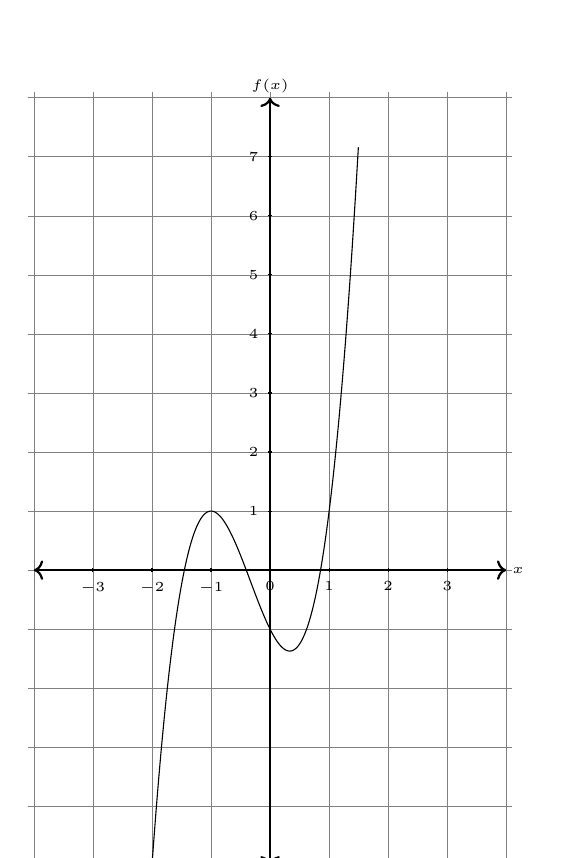
\begin{tikzpicture}[scale = 0.75]
			\draw[step=1cm,gray,very thin] (-4.1,-5.1) grid (4.1,8.1);
			\draw[thick,->] (0,0) -- (4,0);
			\draw[thick,->] (0,0) -- (0, 8);
			\draw[thick,->] (0,0) -- (0, -5);
			\draw[thick,->] (0,0) -- (-4,0);
			\node[] at (4.2, 0) {\tiny $x$};
			\node[] at (0, 8.2) {\tiny $f(x)$};
			\foreach \x in {-3, ..., 3}
   \draw (\x cm,1pt) -- (\x cm,-1pt) node[anchor=north] {\tiny $\x$};
\foreach \y in {1, ...,7}
    \draw (1pt,\y cm) -- (-1pt,\y cm) node[anchor=east] {\tiny $\y$};

    \draw[variable=\t,domain=-2:1.5,samples=500] plot ({\t},{2*\t*\t*\t + 2*\t*\t - 2*\t - 1});

		\end{tikzpicture}
	\end{center}
	Above is the graph.
		\end{soln}
	\end{itemize}
	%
	\newpage
	\item[11.] Sketch a continuous curve $y = f(x)$ having all the following properties:\\
	$f(-2) = 8,\;f(0) = 4,\;f(2) = 0;\;f'(-2) = f(2) = 0;$\\
	$f'(x) > 0$ for $\md{x} > 2,$ $f'(x) < 0$ for $\md{x} < 2;$\\
	$f''(x) < 0$ for $x < 0$ and $f''(x) > 0$ for $x > 0.$
	\begin{soln} Here is the graph:

		\begin{center}
		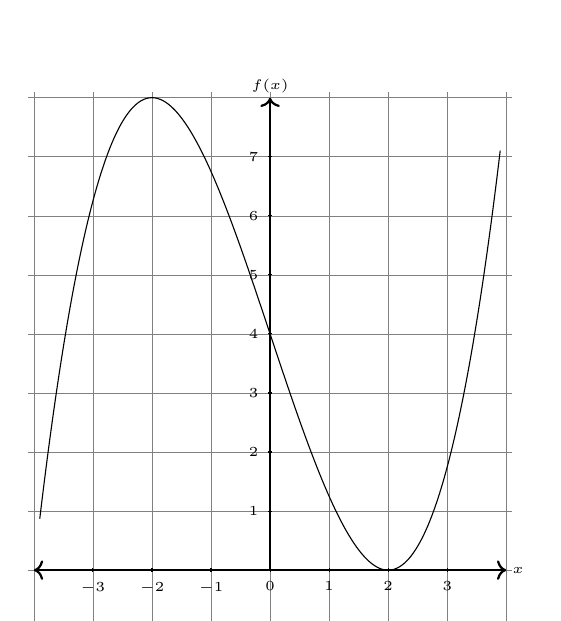
\begin{tikzpicture}[scale = 0.75]
			\draw[step=1cm,gray,very thin] (-4.1,-1.1) grid (4.1,8.1);
			\draw[thick,->] (0,0) -- (4,0);
			\draw[thick,->] (0,0) -- (0, 8);
			\draw[thick,->] (0,0) -- (-4,0);
			\node[] at (4.2, 0) {\tiny $x$};
			\node[] at (0, 8.2) {\tiny $f(x)$};
			\foreach \x in {-3, ..., 3}
		   \draw (\x cm,1pt) -- (\x cm,-1pt) node[anchor=north] {\tiny $\x$};
		\foreach \y in {1, ...,7}
		    \draw (1pt,\y cm) -- (-1pt,\y cm) node[anchor=east] {\tiny $\y$};

		    \draw[variable=\t,domain=-3.9:3.9,samples=500] plot ({\t},{0.25*\t*\t*\t - 3*\t + 4});

		\end{tikzpicture}
	\end{center}
		I have actually graphed a polynomial that satisfies the given properties.\\
		Can you come up with it?\\
		Is there a unique such polynomial?\\
		What's the minimum degree of such a polynomial?\\
		Is there a unique polynomial with that degree?\\
		Suppose you have two distinct polynomials $f$ and $g$ that satisfy the given conditions. Can you come up with a distinct third polynomial such that it satisfies the conditions as well?
	\end{soln}
\end{itemize}
\newpage
\textbf{Sheet 3}
\begin{itemize}
	\item[1.] Write down the Taylor series for $\arctan x$ about the point $0.$ Write down a precise remainder $R_n(x).$
	\begin{soln}
		For each of notation, let $f(x) \vcentcolon= \arctan x$ and $g(x) \vcentcolon= \dfrac{1}{1 + x^2}.$\\
		Note that $f' = g.$

		Note that if $n \ge 1,$ then $f^{(n)}(0) = g^{(n - 1)}(0).$ For $g,$ we have the easy Taylor expansion as
		\begin{equation*} 
			g(x) = 1 - x^2 + x^4 - \cdots
		\end{equation*}
		which is valid for $x \in (-1, 1).$

		Thus, we easily see that
		\begin{equation*} 
			g^{(n)}(0) = \begin{cases}
				0 & n \text{ is odd,}\\
				(-1)^{n/2}n! & n \text{ is even.}
			\end{cases}
		\end{equation*}

		Thus,
		\begin{equation*} 
			f^{(n)}(0) = \begin{cases}
				0 & n \text{ is even,}\\
				(-1)^{(n - 1)/2}(n - 1)! & n \text{ is odd.}
			\end{cases}
		\end{equation*}
		(The above is for $n \ge 1.$)
		Using this, we get the $(2n + 1)$-th Taylor polynomial as
		\begin{align*} 
			P_{2n + 1}(x) &= \sum_{k = 0}^{2n + 1}\dfrac{f^{(n)}(0)}{n!}x^n\\
			&= f(0) + \sum_{k = 1}^{2n + 1}\dfrac{f^{(n)}(0)}{n!}x^n\\
			&= 0 + x - \dfrac{2!}{3!}x^3 + \cdots + \dfrac{(-1)^n(2n)!}{(2n + 1)!}x^{2n + 1}\\
			&= x - \dfrac{x^3}{3} + \cdots + \dfrac{(-1)^n}{2n + 1}x^{2n + 1}.
		\end{align*}
		Since $f^{(2n)} = 0,$ we see that
		\begin{equation*} 
			P_{2n}(x) = P_{2n - 1}(x)
		\end{equation*}
		for $n \ge 1.$

		This solves the problem for finding the Taylor polynomial. Now we solve for the remainder.

		Once again, note that
		\begin{equation*} 
			g(t) = 1 - t^2 + t^4 - \cdots.
		\end{equation*}
		For $n \ge 1,$ we note that
		\begin{align*} 
			g(t) &= [1 - t^2 + \cdots + (-1)^nt^{2n}] + {\color{red}(-1)^{n+1}t^{2n + 2}[1 - t^2 + \cdots]}\\
			&= [1 - t^2 + \cdots + (-1)^nt^{2n}] + {\color{red}(-1)^{n+1}\dfrac{t^{2n + 2}}{1 + t^2}}
		\end{align*}
		Integrating both sides from $0$ to $x$ gives
		\begin{equation*} 
			f(x) = P_{2n + 1}(x) + {\color{red}(-1)^{n+1}\int_{0}^{x} \dfrac{t^{2n + 2}}{1 + t^2} {\mathrm{d}}t}.
		\end{equation*}
		Thus, the term in red is the $(2n + 1)$-th remainder $R_{2n + 1}(x).$ Conclude as before, for $R_{2n}(x).$
	\end{soln}
	%
	\newpage
	\item[2.]  Write down the Taylor series of the polynomial $x^3 - 3x^2 + 3x - 1$ about the point $1.$
	\begin{soln}
		As one can easily calculate, we have
		\begin{equation*} 
			f^{(n)}(1) = \begin{cases}
				6 & n = 3\\
				0 & n \neq 3,
			\end{cases}
		\end{equation*}
		for $n \ge 0.$ Thus, we get the Taylor ``series'' to actually be the following finite sum:
		\begin{equation*} 
			\dfrac{f^{(3)}(1)}{3!}(x - 1)^3.
		\end{equation*}
		In other words, the Taylor series is simply $(x - 1)^3.$
	\end{soln}
	%
	\newpage
	\item[4.] Consider the series $\sum_{k = 0}^{\infty}\frac{x^k}{k!}$ for a fixed $x.$ Prove that it converges as follows. Choose $N > 2\md{x}.$ We see that for all $n > N,$
	\begin{equation*} 
		\dfrac{x^{n + 1}}{(n + 1)!} \le \dfrac{1}{2}\dfrac{\md{x}^n}{n!}.
	\end{equation*}
	It should now be relatively easy to show that the given series is Cauchy, and hence (by the completeness of $\mathbb{R}$), convergent.
	\begin{soln}
		If $N > 2\md{x}$ and $n > N,$ then
		\[\begin{WithArrows}[displaystyle]
			\md{\dfrac{x^{n+1}}{(n + 1)!}} &= \md{\dfrac{x^n}{n!}}\md{\dfrac{x}{n+1}} \Arrow{$n + 1 > n > N$}\\
			&\le \md{\dfrac{x^n}{n!}}\md{\dfrac{x}{N}} \Arrow{$N > 2\md{x}$}\\
			&\le \dfrac{1}{2}\md{\dfrac{x^n}{n!}}.
		\end{WithArrows}\]
		Thus, we can repeatedly use the above to get:
		\begin{equation*} 
			\md{\dfrac{x^{n+1}}{(n + 1)!}} \le \dfrac{1}{2}\md{\dfrac{x^n}{n!}} \le \cdots \le \dfrac{1}{2^{n + 1 - N}}\md{\dfrac{x^N}{N!}}.
		\end{equation*}
		Let $s_n(x) = \displaystyle\sum_{k = 0}^{n}\dfrac{x^k}{k!}.$


		Now, given $m > n > N,$ we have
		\begin{align*} 
			\md{s_m(x) - s_n(x)} &= \md{\sum_{k = n+1}^{m}\dfrac{x^k}{k!}}\\
			&\le \sum_{k = n + 1}^{m}\md{\dfrac{x^k}{k!}}\\
			&= \md{\dfrac{x^{n + 1}}{(n + 1)!}} + \cdots + \md{\dfrac{x^m}{m!}}\\
			&\le \dfrac{\md{x}^N}{N!}\left(\dfrac{1}{2} + \cdots + \dfrac{1}{2^{m-n}}\right)\\
			&{\color{myupdatecolor}\le} \dfrac{\md{x}^N}{N!}.
		\end{align*}
		Note that given any $\epsilon > 0,$ we can pick $N \in \mathbb{N}$ such that $\dfrac{\md{x}^N}{N!} < \epsilon.$ Conclude Cauchy-ness.
	\end{soln}
	%
	\newpage
	\item[5.] Using Taylor series, write down a series for 
	\begin{equation*} 
		\int \dfrac{e^x}{x} {\mathrm{d}}x.
	\end{equation*}
	\begin{soln}
		Note that
		\begin{equation*} 
			e^x = 1 + \sum_{k = 1}^{\infty}\dfrac{x^k}{k!}.
		\end{equation*}
		Dividing by $x$ gives
		\begin{equation*} 
			\dfrac{e^x}{x} = \dfrac{1}{x} + \sum_{k = 1}^{\infty}\dfrac{x^{k-1}}{k!}.
		\end{equation*}
		Integrating both sides gives us
		\begin{equation*} 
			\int \dfrac{e^x}{x} {\mathrm{d}}x = C + \log x + \sum_{k = 1}^{\infty}\dfrac{x^{k}}{k\cdot k!}
		\end{equation*}
	\end{soln}
\end{itemize}
%
%
%

\newpage\section{Tutorial 4}
\begin{center}
	16th December, 2020
\end{center}
\textbf{Sheet 4}
\begin{itemize}
	\item[2.] \begin{itemize}
		\item[(a)] Let $f:[a, b] \to \mathbb{R}$ be Riemann integrable and $f(x) \ge 0$ for all $x \in [a, b].$ Show that $\displaystyle\int_{a}^{b} f(x) {\mathrm{d}}x \ge 0.$ Further, if $f$ is continuous and $\displaystyle\int_{a}^{b} f(x) {\mathrm{d}}x = 0,$ show that $f(x) = 0$ for all $x \in [a, b].$
		\begin{soln}
			For the first part, let 
			\begin{equation*} 
				P = \{a = x_0 < x_1 < \cdots < x_n = b\}
			\end{equation*}
			be an arbitrary partition of $[a, b].$ Note that
			\begin{equation*} 
				m_i = \inf_{x \in [x_i, x_{i + 1}]}f(x) \ge 0
			\end{equation*}
			for all $0 \le i \le n - 1.$ (This is because $0$ is a lower bound of $f.$)

			Thus, we get that $L(f, P) \ge 0.$

			In turn, we see that $L(f) \ge 0,$ since $L(f)$ is the supremum of $L(f, P)$ over \underline{all} partitions $P$ of $[a, b].$ Since $f$ is given to be Riemann integrable, we know that the integral is $L(f)$ and we are done.
			
			\hrulefill
			
			For the second part, we prove by contrapositive. That is, if $f(x) \neq 0$ for some $x \in [a, b],$ then $\displaystyle\int_{a}^{b} f(x) {\mathrm{d}}x \neq 0.$

			Suppose $c \in [a, b]$ is such that $f(c) \neq 0.$ As $f(x) \ge 0$ for all $x \in [a, b],$ we have that $f(c) > 0.$ Let $\epsilon \vcentcolon= f(c).$

			As $f$ is continuous, there is a $\delta > 0$ such that if $x \in [a, b]$ and $|x - c| < \delta,$ then $|f(x) - f(c)| < \epsilon/2$ which implies that $\epsilon/2 < f(x).$

			Note that even if $c = a$ or $c = b,$ the above shows that we can find $c \in (a, b)$ with $f(c) > 0.$ Thus, WLOG we may assume that $c \in (a, b).$ Moreover, we may also assume that $\delta > 0$ is small enough so that $(c- \delta, c + \delta) \subset (a, b).$

			Now, consider the partition of $[a, b]$ given as
			\begin{equation*} 
				P = \{a, c - \delta/2, c + \delta/2, b\}.
			\end{equation*}
			Now, note that
			\begin{equation*} 
				\inf_{x \in [c - \delta/2, c + \delta/2]} f(x) \ge \dfrac{\epsilon}{2}.
			\end{equation*}

			Thus, $L(P, f) > 0.$ As $L(f)$ is the supremum over all such $L(P, f),$ we see that $L(f) > 0.$ Since $f$ is given to be Riemann integrable, we know that the integral is $L(f)$ and we are done.
		\end{soln}
		%
		\item[(b)] Give an example of a Riemann integrable function on $[a, b]$ such that $f(x)	\ge 0$ for all $x \in [a, b]$ and $\displaystyle\int_{a}^{b} f(x) {\mathrm{d}}x = 0,$ but $f(x) \neq 0$ for some $x \in [a, b].$
		\begin{soln}
			Let $a = 0, b = 2$ and $f:[a, b] \to \mathbb{R}$ be defined as
			\begin{equation*} 
				f(x) \vcentcolon= \begin{cases}
					0 & x \neq 1,\\
					1 & x = 1.
				\end{cases}
			\end{equation*}
			Show that $f$ is actually Riemann integrable on $[0, 2]$ with the integral equal to $0.$
		\end{soln}
	\end{itemize}
	%
	%
	\newpage
	\item[3] Evaluate $\displaystyle\lim_{n\to \infty}S_n$ by showing that $S_n$ is an appropriate Riemann sum for a suitable function over a suitable interval.

	\begin{itemize}
		\item[(ii)] $S_n = \sum_{i = 1}^{n}\dfrac{n}{i^2 + n^2}.$
		\item[(iv)] $S_n = \dfrac{1}{n}\sum_{i = 1}^{n}\cos\left(\dfrac{i\pi}{n}\right).$
	\end{itemize}

	\begin{soln}
		For both the parts, we shall use the following theorem:
		
		\begin{thm}
			Let $f:[a, b] \to \mathbb{R}$ be Riemann integrable. Suppose that $(P_n, t_n)$ is a sequence of tagged partitions of $[a, b]$ such that $\|P_n\| \to 0.$\\
			Then,
			\begin{equation*} 
				\lim_{n\to \infty}R(f, P_n, t_n) = \int_{a}^{b} f(x) {\mathrm{d}}x.
			\end{equation*}
		\end{thm}

		Note very carefully in the above that we already need to know that $f$ is Riemann integrable.

		\begin{itemize}
			\item[(ii)] Note that 
			\begin{equation*} 
				S_n = \sum_{i=1}^{n}\dfrac{n}{i^2 + n^2} = \sum_{i=1}^{n}\dfrac{1}{\left(\frac{i}{n}\right)^2 + 1}\left(\frac{i}{n} - \frac{i-1}{n}\right).
			\end{equation*}
			Define $f:[0, 1] \to \mathbb{R}$ by $f(x) \vcentcolon= \tan^{-1}x.$\\
			Then, we have that $f'(x) = \dfrac{1}{x^2 + 1}.$

			As $f'$ is continuous and bounded, it is (Riemann) integrable. \\
			For $n \in \mathbb{N},$ let 
			\begin{equation*} 
				P_n \vcentcolon= \{0, 1/n, \ldots, n/n\}
			\end{equation*} and tags 
			\begin{equation*} 
				t_i \vcentcolon= i/n
			\end{equation*} for $i = 1, 2, \ldots, n.$

			Then, $S_n = R(f', P_n, t_n).$ Since $\|P_n\| = 1/n \to 0,$ it follows that
			\begin{equation*} 
				\lim_{n\to \infty}R(f, P_n, t_n) = \int_{0}^{1} \dfrac{1}{x^2 + 1} {\mathrm{d}}x = \int_{0}^{1} f'(x) {\mathrm{d}}x.
			\end{equation*}
			By FTC Part II, we have it that
			\begin{equation*} 
				\lim_{n\to \infty}S_n = \int_{0}^{1} f'(x) {\mathrm{d}}x = f(1) - f(0) = \dfrac{\pi}{4}.
			\end{equation*}
			%
			\item[(iv)] Note that 
			\begin{equation*} 
				S_n = \dfrac{1}{n}\sum_{i=1}^{n}\cos\left(\dfrac{i\pi}{n}\right) = \sum_{i=1}^{n}\cos\left(\dfrac{i\pi}{n}\right)\left(\frac{i}{n} - \frac{i-1}{n}\right).
			\end{equation*}
			Define $f:[0, 1] \to \mathbb{R}$ by $f(x) \vcentcolon= \pi^{-1}\sin(\pi x).$\\
			Then, we have that $f'(x) = \cos(\pi x).$

			As $f'$ is continuous and bounded, it is (Riemann) integrable. \\
			For $n \in \mathbb{N},$ let 
			\begin{equation*} 
				P_n \vcentcolon= \{0, 1/n, \ldots, n/n\}
			\end{equation*} and tags 
			\begin{equation*} 
				t_i \vcentcolon= i/n
			\end{equation*} for $i = 1, 2, \ldots, n.$

			Then, $S_n = R(f', P_n, t_n).$ Since $\|P_n\| = 1/n \to 0,$ it follows that
			\begin{equation*} 
				\lim_{n\to \infty}R(f, P_n, t_n) = \int_{0}^{1} \cos(\pi x) {\mathrm{d}}x = \int_{0}^{1} f'(x) {\mathrm{d}}x.
			\end{equation*}
			By FTC Part II, we have it that
			\begin{equation*} 
				\lim_{n\to \infty}S_n = \int_{0}^{1} f'(x) {\mathrm{d}}x = f(1) - f(0) = 0. \qedhere
			\end{equation*}
		\end{itemize}
	\end{soln}
	%
	%
	%
	%
	\newpage
	\item[4. (b)] Compute $F'(x),$ if for $x \in \mathbb{R}$
	\begin{itemize}
		\item[(i)] $F(x) = \displaystyle\int_{1}^{2x} \cos(t^2) {\mathrm{d}}t.$
		\item[(ii)] $F(x) = \displaystyle\int_{0}^{x^2} \cos(t) {\mathrm{d}}t.$
	\end{itemize}

	\begin{soln}
		For both the parts, we shall use the following theorem:
		
		\begin{thm}
			Let $v:\mathbb{R} \to \mathbb{R}$ be differentiable and $g:\mathbb{R}\to\mathbb{R}$ be continuous. Suppose that $F:\mathbb{R}\to\mathbb{R}$ is defined by
			\begin{equation*} 
				F(x) \vcentcolon= \int_{0}^{v(x)} g(t) {\mathrm{d}}t.
			\end{equation*}
			Then,
			\begin{equation*} 
				F'(x) = g(v(x))v'(x).
			\end{equation*}
		\end{thm}
		Note that using the above, we can state the more general result for when the lower limit is also a differentiable function.

		\begin{proof} 
			First, define $G:\mathbb{R}\to\mathbb{R}$ by
			\begin{equation*} 
				G(x) \vcentcolon= \int_{0}^{x} g(t) {\mathrm{d}}t.
			\end{equation*}
			By FTC Part I, we know that $G$ is differentiable and
			\begin{equation*} 
				G'(x) = g(x).
			\end{equation*}
			On the other hand, note that
			\begin{equation*} 
				F(x) = G(v(x)).
			\end{equation*}
			An application of chain rule yields
			\begin{equation*} 
				F'(x) = G'(v(x))v'(x) = g(v(x))v'(x). \qedhere
			\end{equation*}
		\end{proof}

		Both the parts are now solved easily.
		\begin{itemize}
			\item[(i)] We have $g(t) = \cos(t^2)$ and $v(x) = 2x.$ Thus, $v'(x) = 2$ and 
			\begin{equation*} 
				\boxed{F'(x) = 2\cos(4x^2).}
			\end{equation*}
			%
			\item[(ii)] We have $g(t) = \cos(t)$ and $v(x) = x^2.$ Thus, $v'(x) = 2x$ and 
			\begin{equation*} 
				\boxed{F'(x) = 2x\cos(x^2).} \qedhere
			\end{equation*}
		\end{itemize}
	\end{soln}
	%
	%
	%
	%
	\newpage
	\item[6.] Let $f:\mathbb{R} \to \mathbb{R}$ be continuous and $\lambda \in \mathbb{R},\; \lambda \neq 0.$ For $x \in \mathbb{R},$ let
	\begin{equation*} 
		g(x) = \dfrac{1}{\lambda}\int_{0}^{x} f(t)\sin\left[\lambda(x - t)\right] {\mathrm{d}}t.
	\end{equation*}
	Show that $g''(x) + \lambda^2g(x) = f(x)$ for all $x \in \mathbb{R}$ and $g(0) = 0 = g'(0).$

	\begin{soln}
		Just brute calculation. Note that
		\begin{align*}
			g(x) &= \dfrac{1}{\lambda}\int_{0}^{x} f(t)\sin \lambda(x - t) {\mathrm{d}}t\\
			&= \dfrac{1}{\lambda}\int_{0}^{x} f(t) \left(\sin \lambda x\cos \lambda t - \cos \lambda x \sin \lambda t\right) {\mathrm{d}}t\\
			&= \frac{1}{\lambda}\sin\lambda x\int_{0}^{x} f(t)\cos \lambda t {\mathrm{d}}t - \frac{1}{\lambda}\cos \lambda x \int_{0}^{x} f(t)\sin \lambda t {\mathrm{d}}t.
		\end{align*}

		Now, we can differentiate $g$ using product rule and FTC Part I.
		\begin{align*}
			g'(x) &= \cos\lambda x\int_{0}^{x} f(t)\cos \lambda t {\mathrm{d}}t + \sin \lambda x \int_{0}^{x} f(t)\sin \lambda t {\mathrm{d}}t \\
		\end{align*}

		Since the limits of integrals appearing in the expressions for $g$ and $g'$ are both from $0$ to $x,$ we see that $g(0) = 0 = g'(0).$

		We can differentiate $g'$ in a similar way and get,
		\begin{align*}
			g''(x) &= -\lambda\sin\lambda x\int_{0}^{x} f(t)\cos \lambda t dt + f(x)\cos^2\lambda x + \lambda \cos \lambda x \int_{0}^{x} f(t)\sin \lambda t dt \\
			& + f(x)\sin^2 \lambda x\\
			&= f(x) - \lambda^2\left(\dfrac{1}{\lambda}\int_{0}^{x} f(t) \left(\sin \lambda x\cos \lambda t - \cos \lambda x \sin \lambda t\right) dt\right)\\
			&= f(x) - \lambda^2g(x).
		\end{align*}
		Rearranging the above gives
		\begin{equation*} 
			g''(x) + \lambda^2g(x) = f(x) \qedhere
		\end{equation*}
	\end{soln}
\end{itemize}
\end{document}